\subsection{Example Based Super Resolution}
\noindent
Como puede observarse la interpolación soluciona parcialmente el problema de
\emph{Súper Resolución}, pero tiene como consecuencia los efectos mencionados. En
particular, el desenfoque resulta contraproducente al intentar mejorar los 
detalles de una imagen. Por lo mismo, en los algoritmos clásicos de \emph{Súper Resolución}
se utiliza la interpolación únicamente para aumentar la densidad de los pixeles
y aproximar la imagen de salida como una imagen más grande con un determinado 
factor de escalado, pero con los detalles de desenfoque que producen los 
algoritmos de interpolación no adaptativos. 

Para solucionarlo, algunos autores proponen realizar un postprocesado a la imagen 
interpolada para incluir los detalles faltantes y con ello mejorar visiblemente 
la resolución de los bordes de la imagen. 

En particular, \cite{freeman} propone un parchado de la imagen reescalada a partir
de un conjunto de entrenamiento o diccionario de parches en pares de alta
y baja resolución. Dichos parches permiten construir una imagen con frecuencias
altas que no están en la imagen de entrada con el objetivo de sumar la imagen
original interpolada con las frecuencias altas que buscan mejorar su resolución
al realzar sus detalles. En la Figura \ref{fig:fr_algoritmo} puede observarse de
manera específica el algoritmo propuesto basado en el parchado de la imagen de 
entrada mediante un algoritmo de predicción.

\begin{figure}[H]
    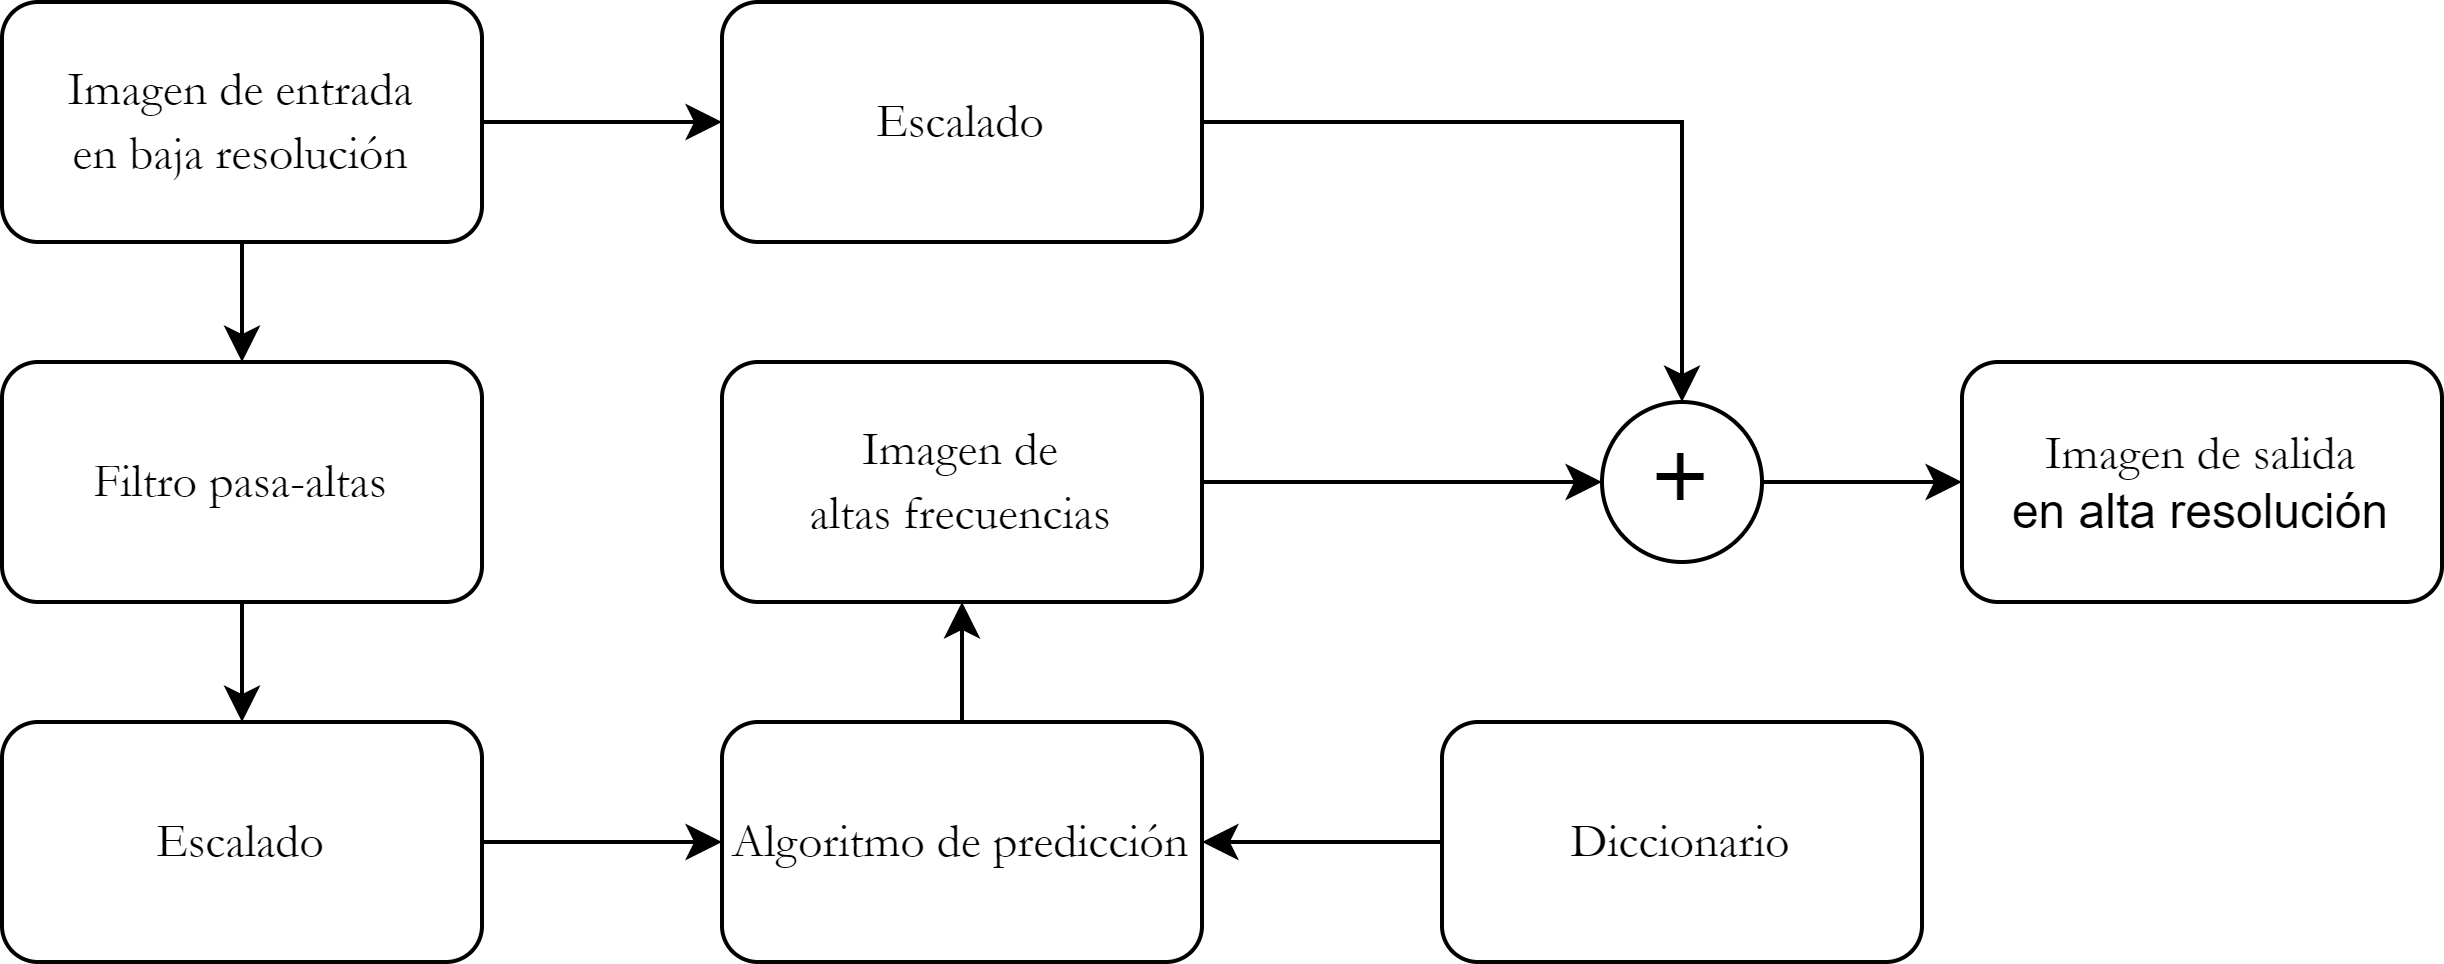
\includegraphics[scale = 0.4]{ fr_algoritmo.png }
    \centering
    \caption{ Algoritmo de súper resolución }
    \label{fig:fr_algoritmo}
\end{figure}

\subsubsection{Diccionario}
\noindent
El algoritmo de \emph{Súper Resolución} \cite{freeman}
opera bajo la premisa que la relación
de predicción entre los parches de alta y baja resolución es independiente del 
contraste de la imagen. Esto también resulta ventajoso, ya que el diccionario 
no necesita ser de imágenes similares a las que se van a reconstruir para 
mejorar la calidad de resolución tal como comenta \cite{diccionario_shuji}.
Esto resulta en un algoritmo general aplicable a cualquier tipo de imagen
y escalable respecto al tamaño de la base de entrenamiento.

Desde el punto de vista de almacenamiento, los parches de baja resolución carecen 
de detalle y por lo tanto predominan las frecuencias bajas, las cuales son 
irrelevantes en su uso para la predicción de detalles y por lo tanto resulta
información necesaria dentro del proceso. Por lo mismo, es aconsejable aplicar un filtro pasa-altas a cada parche 
con el objetivo de dejar sólo la información útil para el algoritmo (detalles).

Por otra parte, para que el diccionario sea funcional sin importar el 
tipo de imagen a reconstruir, se busca normalizar cada pareja de parche con el 
objetivo de mantener su relación intrínseca. De acuerdo con \cite{freeman}, 
los parches de baja resolución se recomiendan con un tamaño de 7x7 pixeles
mientras que los de alta resolución serán de 5x5 todos con centro en el mismo pixel
para mantener la relación tal como se presenta en la Figura \ref{fig:fr_dic}.

\begin{figure}[H]
    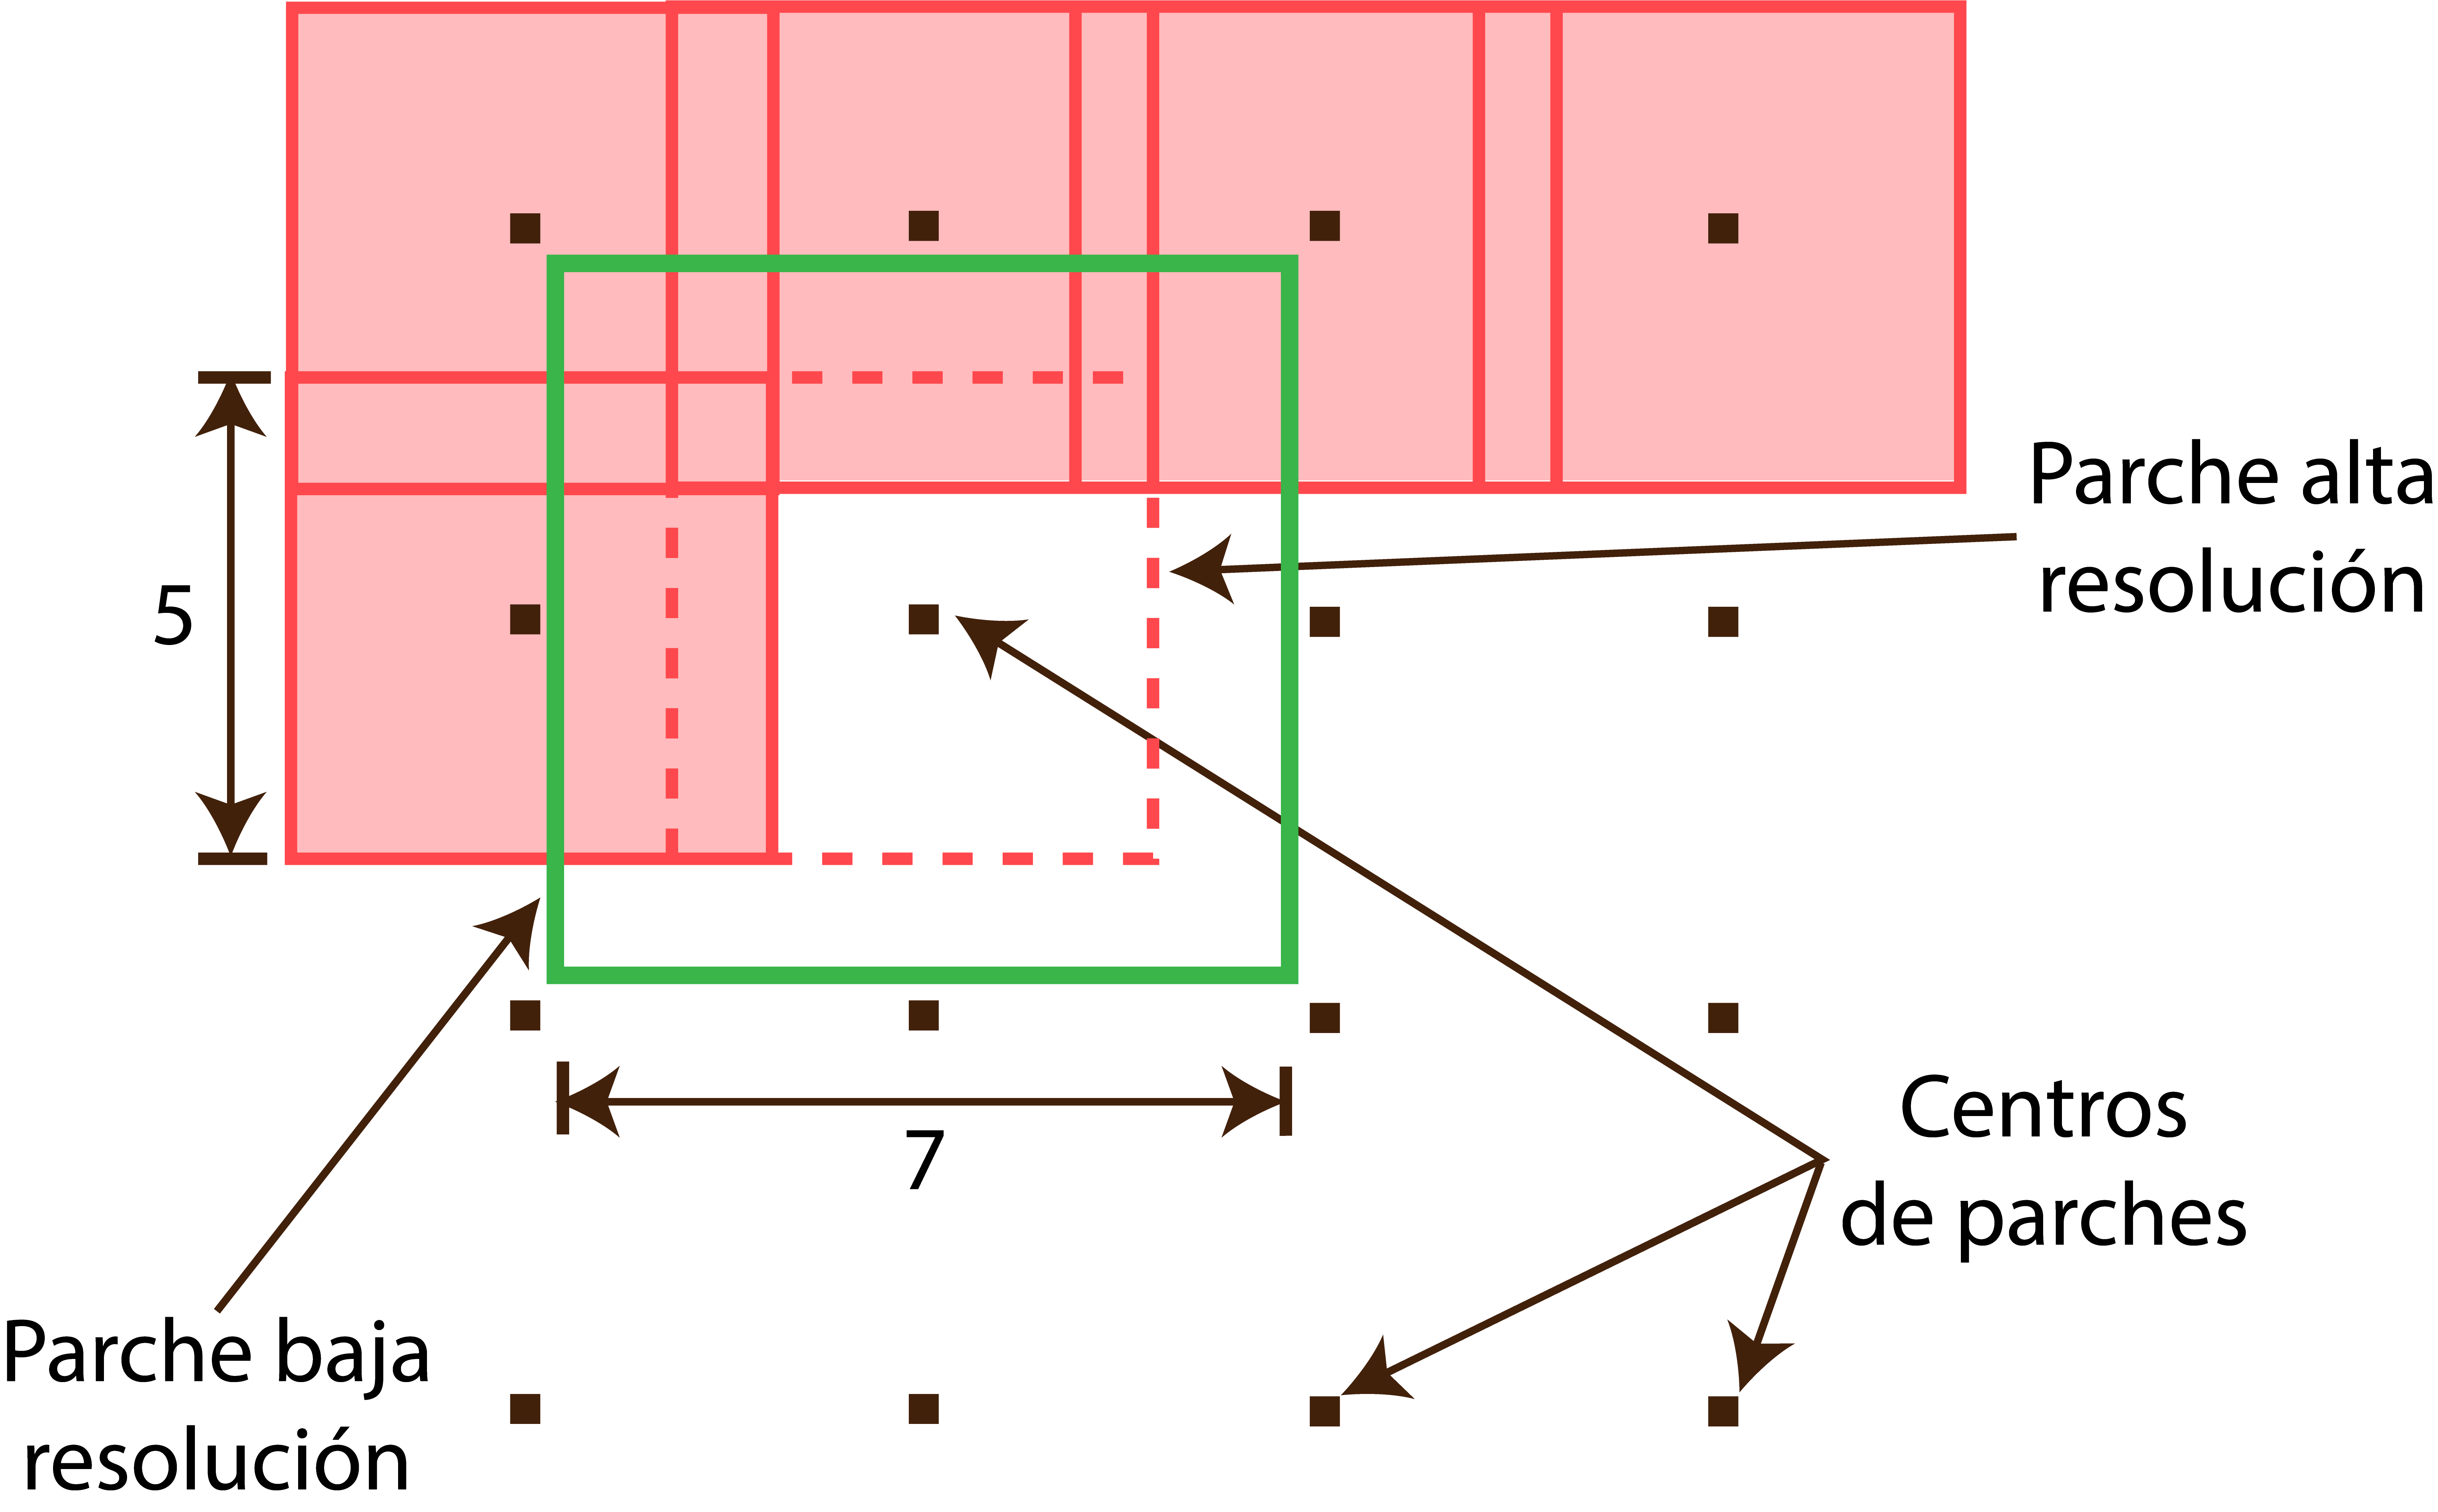
\includegraphics[scale = 0.3]{ fr_diccionario.png }
    \centering
    \caption{ Adquisición de parches de cada imagenes}
    \label{fig:fr_dic}
\end{figure}

En específico, los parches de baja resolución deben reordenarse como un vector 
en $\mathbb{R}^{1\times49}$ concatenado con la primera fila y primera columna
del parche de alta resolución, resultando en un vector en $\mathbb{R}^{1\times59}$.
Lo último es necesario para considerar la superposición
de los parches de alta resolución de la imagen a reconstruir. 

Cabe destacar que la base de entrenamiento está en 
RGB por lo que bastará con el procedimiento antes mencionado para guardar
los pares de parches en algún archivo de fácil acceso. 

\subsubsection{Algoritmo de predicción}
\noindent
Una vez teniendo el diccionario o base de entrenamiento es necesario establecer el algoritmo de 
predicción para generar esos detalles no visibles en la imagen original.
Para ello, la imagen de entrada (en baja resolución) debe ser pre-procesada
mediante un filtro pasa-altas para eliminar información innecesaria y posteriormente realizar
un proceso de escalado mediante algún algoritmo de interpolación para
aumentar sus dimensiones y densidad de los pixeles tal como se presenta
en la Figura \ref{fig:fr_algoritmo}. Observe que para ese punto, la imagen de entrada
cuenta con los píxeles que representan sus bordes o detalles que han sido
escalados con el objetivo de tener una base a partir de la cual se va a reconstruir
con más detalle la imagen de salida.  

Puesto que \cite{freeman} propone que la reconstrucción sea con parches, se debe 
realizar una búsqueda para elegir al parche de la base de datos que se aproxime 
más al parche de entrada con el objetivo de realizar la reconstrucción. En la
Figura \ref{fig:fr_prediccion} se observa el algoritmo propuesto por
\emph{Freeman et al} para la predicción de parches.

\begin{figure}[H]
    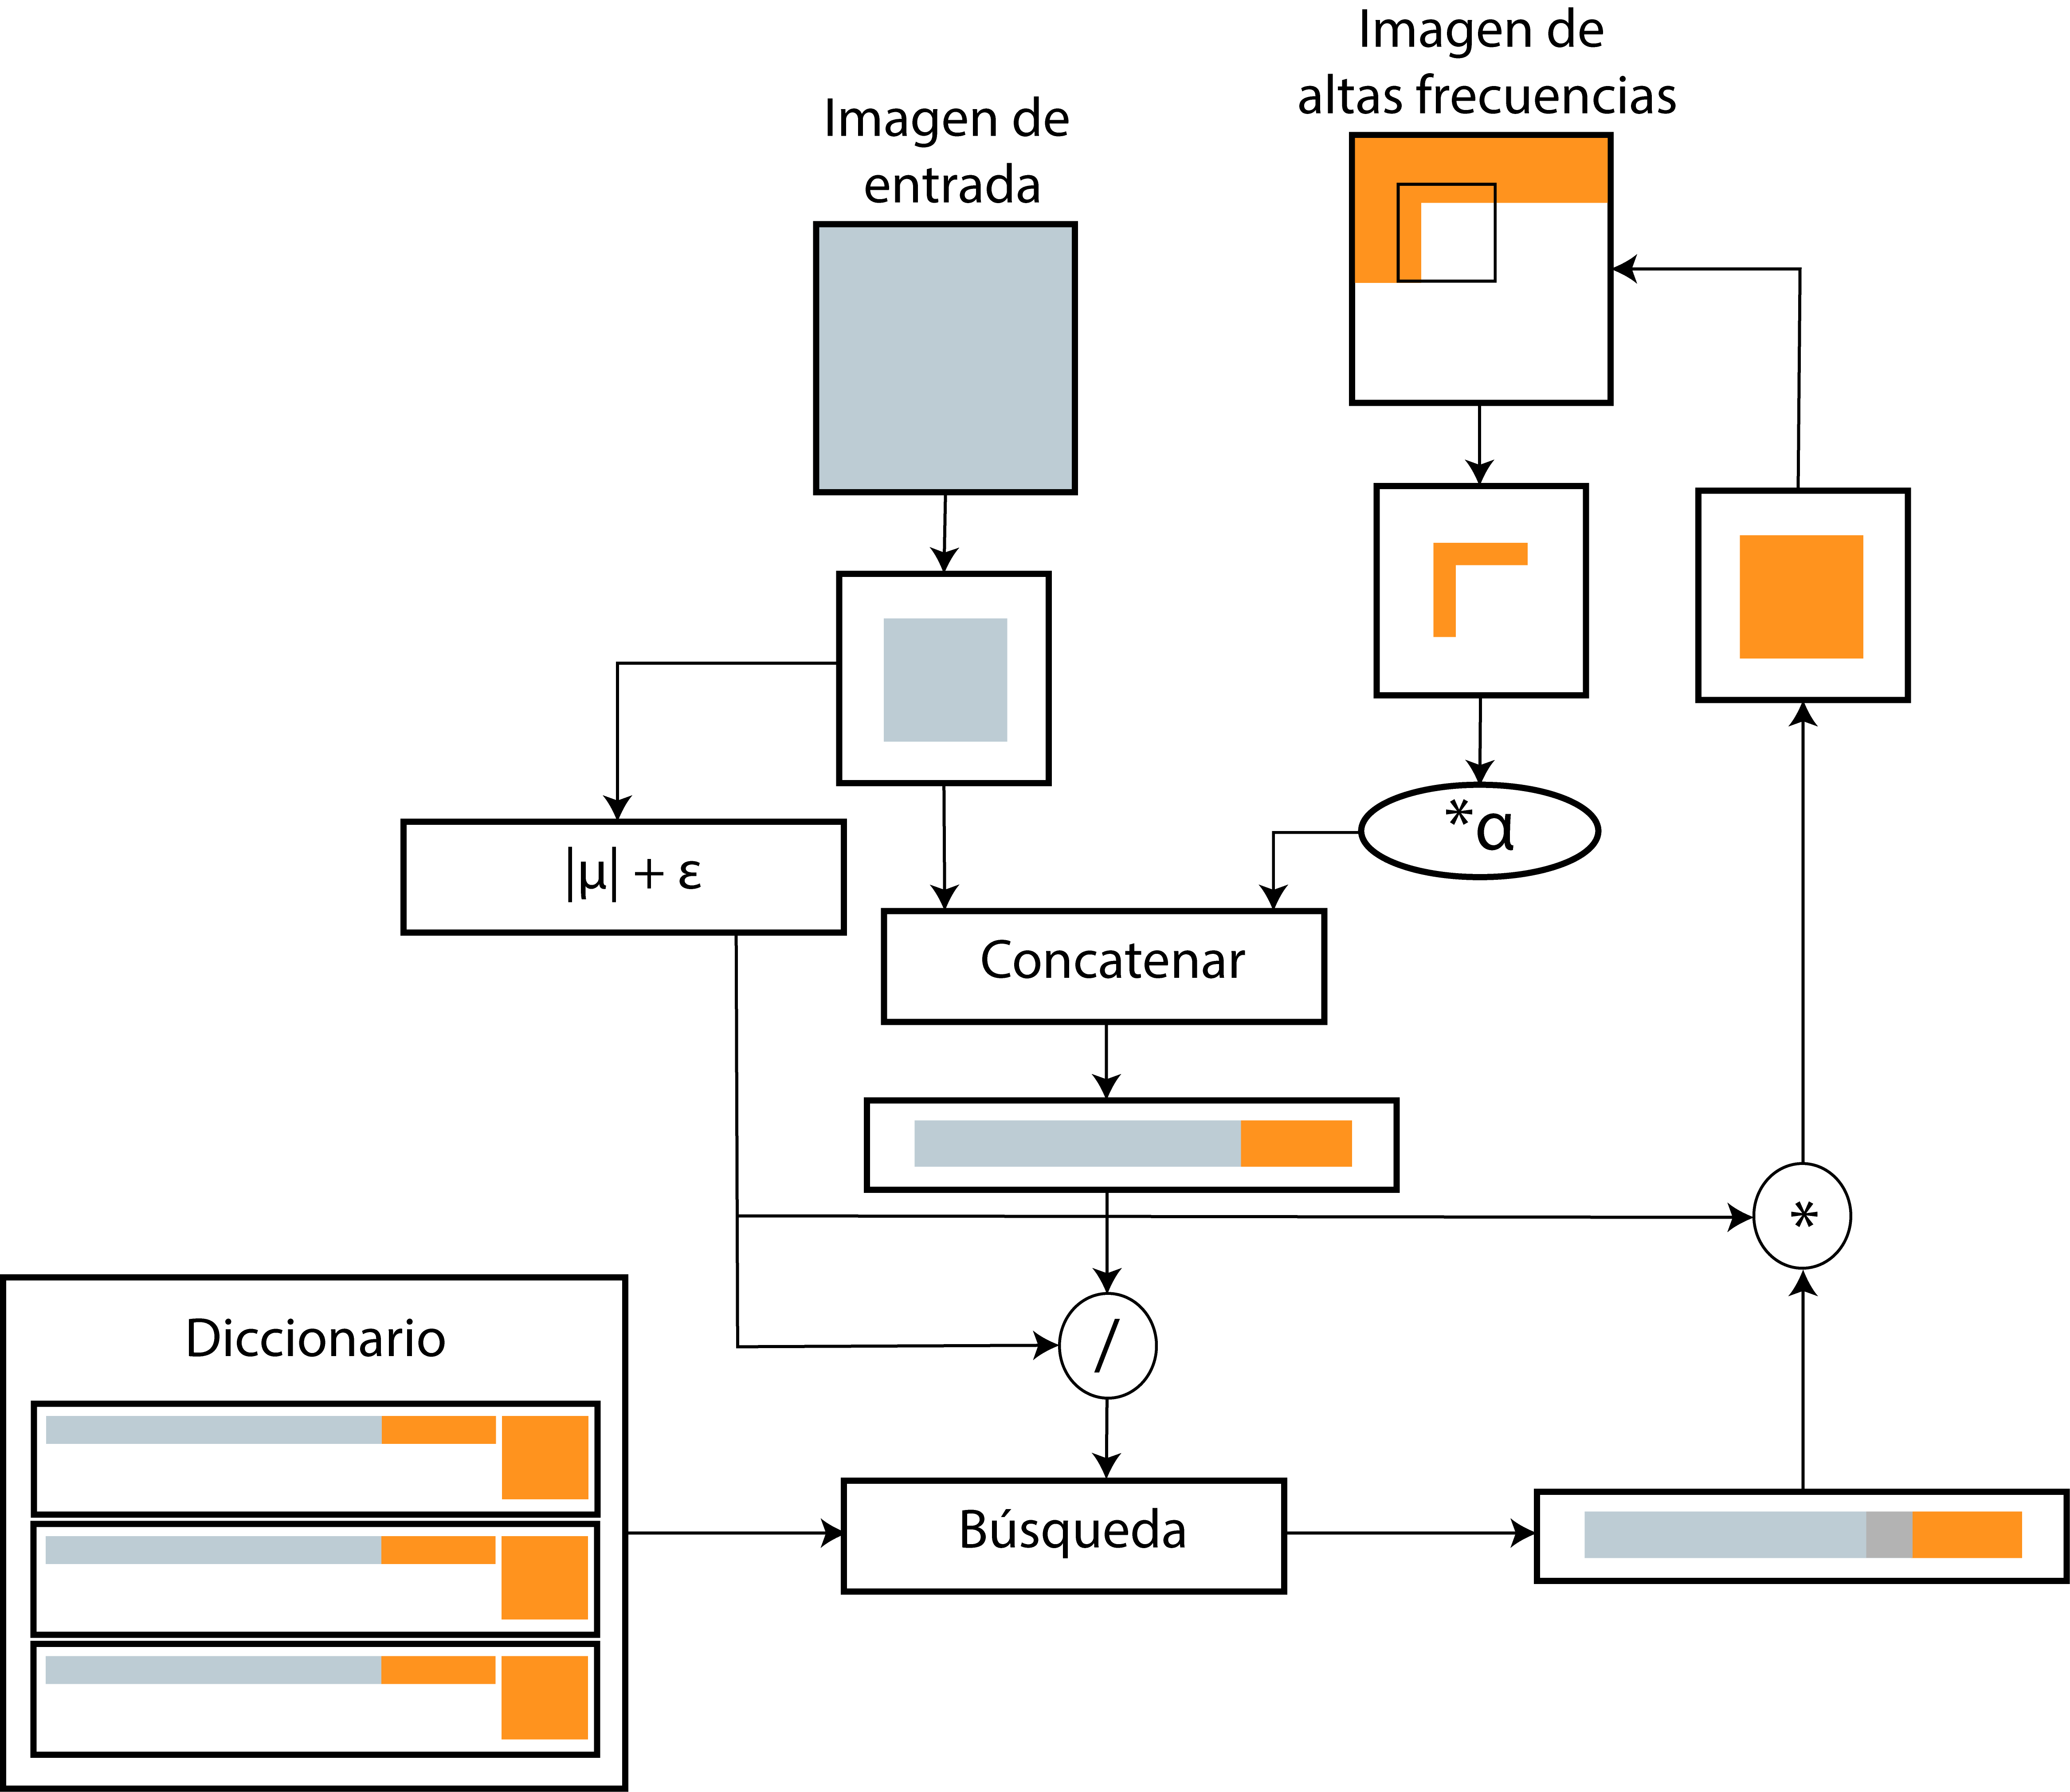
\includegraphics[scale = 0.5]{ freeman_prediccion.png}
    \centering
    \caption{ Algoritmo de predicción de imagen de frecuencias altas }
    \label{fig:fr_prediccion}
\end{figure}

Observe que la imagen de entrada se irá segmentando en los parches de baja 
resolución (color gris-verdoso). Estos parches se calculará su media absoluta 
$|\mu|$ más un $\epsilon$ (para evitar indeterminación ante parches con poco
contraste), posteriormente se concatena con el producto del factor de control 
$\alpha$ que considera la \emph{superposición} entre los parches de alta resolución
(naranjas). Dicha concatenación se divide entre el promedio absoluto más $\epsilon$
para convertirse en el vector a buscar en el diccionario. 

Dada la gran combinación de valores, resulta bastante complicado encontrar 
exactamente el mismo vector en el diccionario previamente construido y por
lo mismo se utilizan algoritmos de búsqueda aproximados como el del \emph{vecino
más cercano}. Esto puede observarse en la salida del algoritmo al notar que el 
vector emparejado tiene un pixel de color diferente al solicitado, pero como 
es muy cercano, resulta la salida del algoritmo de búsqueda. 

Dicho vector de búsqueda permite emparejar al parche de alta resolución asociado
en el diccionario, el cual será multiplicado por el factor $|\mu|+\epsilon$ para 
retomar las tonalidades del parche de baja resolución e incrustado en la \emph{imagen de altas frecuencias}
para ejecutar nuevamente el algoritmo de manera iterativa.

De acuerdo con \cite{freeman}, el \emph{algoritmo de un paso} evita considerar
los parches como variables aleatorias y relacionarlas con \emph{Redes de Markov}
considerando el algoritmo \emph{belief propagation}. Esto es una enorme ventaja,
ya que se simplifica el proceso de selección del parche considerando 
únicamente la \emph{superposición} futura en los parches de alta resolución. 

\subsubsection{Imagen de alta resolución}
\noindent
Finalmente, como resultado del algoritmo propuesto en \cite{freeman} se obtiene
una imagen de mejor resolución que la entrada considerando un factor de escalado
deseado para el proceso de interpolación. Note que el motor central del algoritmo
está basado en el algoritmo de predicción descrito anteriormente y el diccionario
construido a partir de un conjunto de imágenes donde se realizará la búsqueda
mediante el algoritmo del \emph{vecino más cercano}. 

Como producto del algoritmo de predicción se obtendrá una imagen con sólo frecuencias
altas que no se encontraban explícitamente en la imagen de entrada y que se sumará
con la imagen escalada para obtener así la imagen de alta resolución respecto
la imagen de entrada tal como se observa en la Figura \ref{fig:fr_algoritmo}.